\documentclass[12pt,a4paper,two column]{article}
\usepackage[utf8]{inputenc}
\usepackage{mathtools}
\usepackage[a4paper, total={6in, 8in}, margin = 1in]{geometry}
\usepackage{enumitem}
\usepackage{graphicx}
\graphicspath{{images/}}
\usepackage{amsmath}

\title{ASSIGNMENT 2}
\author{Abhishek Kumar \\AI21BTECH11003}
\date{April 2022}
\begin{document}
	\maketitle
	\section*{Question 1(i)}
	\begin{align}
		&f:R\xrightarrow{} R,f(x)= x^3\\
		&g:R\xrightarrow{} R,g(x)=2x^2+1
	\end{align}
	$R$ is the set of Real Numbers.Find $fog(x)$ and $gof(x)$.
	\section*{Solution}
	Lets find  $fog(x)$
	\begin{align}
		&f(x)=x^3,g(x)=2x^2+1\nonumber\\
		&\implies f(g(x))= (2x^2+1)^3\\
		&\implies fog(x)=8x^6+12x^4+6x^2+1, x\in \mathbb{R}
	\end{align}
	Lets find  $gof(x)$
	\begin{align}
		&f(x)=x^3,g(x)=2x^2+1\nonumber\\
		&\implies g(f(x))= 2(x^3)^2+1\\
		&\implies fog(x)= 2x^6+1,x \in \mathbb{R}
	\end{align}
	\begin{figure}[h]
		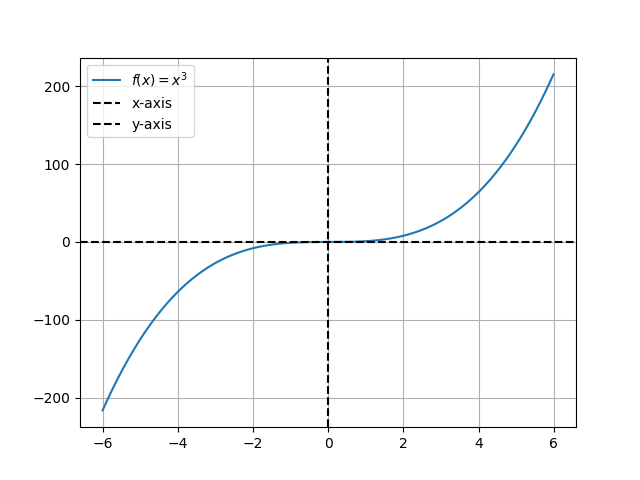
\includegraphics[width = \columnwidth]{f(x)}
		\caption{$f(x)=x^3$}
		\label{fig-1}
	\end{figure}
	\begin{figure}
		\centering
		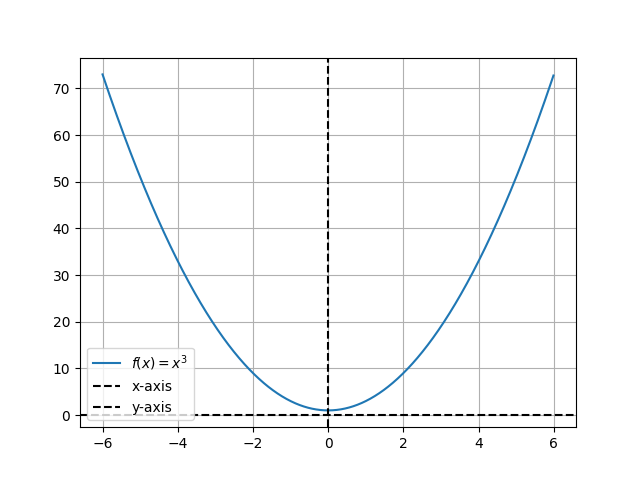
\includegraphics[width=\columnwidth]{g(x).png}
		\caption{$g(x)=2x^2+1$}
		\label{fig-2}
	\end{figure}
	\begin{figure}
		\centering
		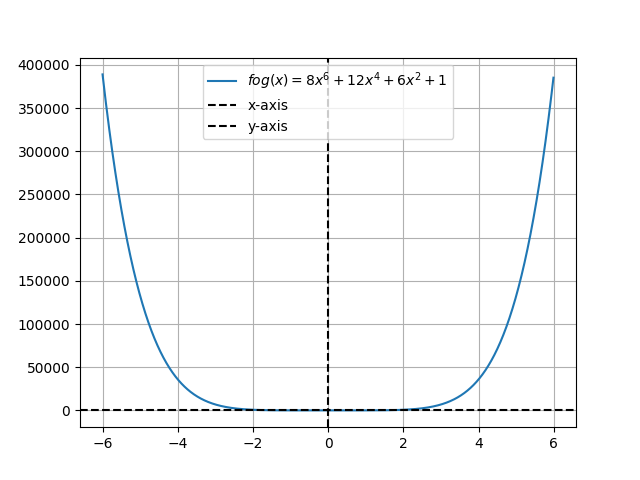
\includegraphics[width=\columnwidth]{fog(x).png}
		\caption{$fog(x)=8x^6+12x^4+6x^2+1$}
		\label{fig-3}
	\end{figure}
	\begin{figure}
		\centering
		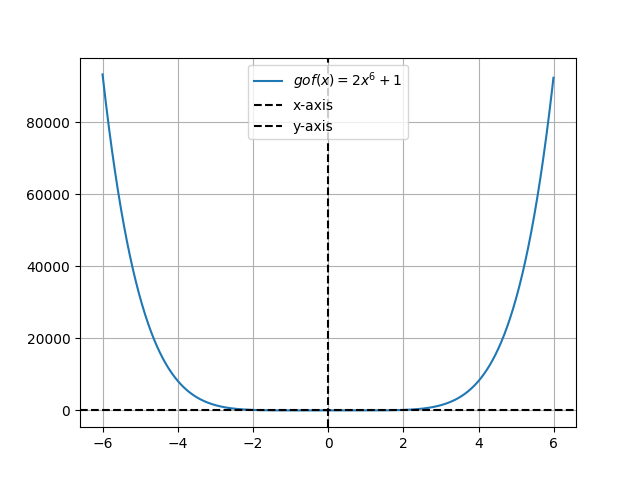
\includegraphics[width=\columnwidth]{gof(x).png}
		\caption{$gof(x)=2x^6+1$}
		\label{fig-4}
	\end{figure}
	
\end{document}
